\section{Planarity and Homomorphism}

Planarity and homomorphism are important concepts in graph theory that help us understand the structure and properties of networks. They provide insights into how networks can be represented and analyzed.

\subsection{Planarity and Genus}
A graph is defined as \textbf{planar} if it can be drawn on a two-dimensional plane without any of its links (edges) crossing each other.

In topological terms, a planar graph has a \textbf{genus} of 0. The genus of a graph represents the minimum number of ``holes'' (or handles on a mathematical manifold, like a torus or a donut) that a surface must have so that the graph can be drawn on it without any intersecting links.

Because links cannot cross, planar graphs face strict structural limitations and must be relatively sparse. Specifically, there is a rigid upper bound: a planar graph with $N$ nodes can have at most $3N-6$ links, meaning the number of links scales linearly, $O(N)$.

To determine if a graph is planar, we rely on \textbf{Kuratowski's Theorem}. This theorem states that a graph is planar if and only if it does not contain any subgraphs that are homomorphic (topologically equivalent) to $K_5$ (the complete graph on 5 nodes) or $K_{3,3}$ (the complete bipartite graph with two sets of 3 nodes).

\subsection{Graph Homomorphism}
A \textbf{graph homomorphism} is a mathematical mapping $f$ from a network $G$ (with $N$ nodes) to a smaller network $G'$ (with $M < N$ nodes) that rigorously preserves node adjacency.

Algebraically, if two nodes $u$ and $v$ are connected in the original graph ($u \sim v$), their mapped counterparts must be connected in the new graph ($f(u) \sim f(v)$):
\[
    G^{\prime} = f(G) \quad \text{with} \quad f: G \rightarrow G^{\prime} \quad \big| \quad u \sim v \implies f(u) \sim f(v).
\]

Practically, a homomorphism acts as a \textbf{dimensionality reduction} for a graph. It simplifies the network by drastically reducing the number of nodes while retaining its essential connectivity patterns and macroscopic characteristics. A classic example is mapping a large network of individual nodes into a smaller homomorphic network of \textbf{communities}: in this new graph, each super-node represents an entire community, and the links show how different communities interact with one another.

\section{Network Reduction and Filtering}

We are often interested in reducing the complexity of a network by filtering out less important links, which can help us to focus on the most relevant connections and to analyze the structure of the network more effectively. This process can be done using various methods, such as minimum spanning trees (MST) or link selection rules based on global or local criteria.

\subsection{Minimum Spanning Tree (MST)}

Let us define a spanning tree as a subgraph of a connected graph that includes all the vertices of the original graph and is a tree (i.e., it is connected and has no cycles) with a special property.

\begin{definition}[Min/Max Spanning Tree]
    A minimum/maximum spanning tree (MST) is a subset of the edges of a connected, weighted graph that connects all the vertices together without any cycles and with the minimum/maximum possible total edge weight. It is a method for finding the most efficient way to connect all the nodes in a graph while minimizing/maximizing the total cost: it finds the backbone of the network.
\end{definition}

The MST can be used in various applications, such as designing efficient communication networks, clustering data, and solving optimization problems. There are several algorithms for finding the MST, including Prim's algorithm and Kruskal's algorithm, which are based on greedy strategies to build the tree incrementally by selecting the edges with the smallest weights.

\paragraph{Kruskal's Algorithm}
Kruskal's algorithm is a greedy, edge-based approach for finding the Minimum Spanning Tree (MST). Instead of growing a single tree, it starts with a "forest" of isolated nodes and connects them using the cheapest available edges that do not violate the tree structure.

\begin{enumerate}
    \item \textbf{Start:} Begin with all nodes as isolated components (a forest) and a list of all edges sorted by weight in non-decreasing order.
    \item \textbf{Iteration:} Iterate through the sorted list of links:
          \begin{itemize}
              \item Consider the link with the minimum weight \( w(e) \).
              \item If the link joins two previously separate trees, add it to the MST.
              \item If the link connects two nodes already in the same component (forming a cycle), \textbf{do not} add it.
          \end{itemize}
    \item \textbf{Removal:} Remove the link from the candidate list and move to the next.
    \item \textbf{Termination:} Continue until the forest is merged into a single spanning tree, which occurs when exactly \( |V|-1 \) edges have been added.
\end{enumerate}

\paragraph{Prim's Algorithm}
Unlike Kruskal's, Prim's algorithm is a node-based greedy approach. It builds the MST by starting from an arbitrary root node and "growing" the tree one node at a time by always choosing the cheapest edge that connects the current tree to a node outside of it.

\begin{enumerate}
    \item \textbf{Start:} Choose a single arbitrary node to begin. Define the set \( V_{MST} \) containing only this root node. Keep a list of all available links in the graph.
    \item \textbf{Iteration:} At each step, identify all edges \( (u, v) \) such that:
          \[
              u \in V_{MST} \quad \text{and} \quad v \notin V_{MST}
          \]
          From this subset of edges, choose the one with the minimum weight \( w(u, v) \).
    \item \textbf{Ties:} If multiple edges share the same minimum weight, select one at random.
    \item \textbf{Update:} Add the new node \( v \) to the set \( V_{MST} \) and remove the used edge from the candidate list.
    \item \textbf{Termination:} Repeat the process until all nodes are included in the set \( V_{MST} \) and the spanning tree is complete.
\end{enumerate}

\begin{remark}
    While both algorithms yield an MST, they differ in execution logic:
    \begin{itemize}
        \item \textbf{Kruskal's} is often more efficient for sparse graphs, as its complexity is dominated by the initial sorting of edges: \( O(E \log E) \).
        \item \textbf{Prim's} can be faster for dense graphs, especially when implemented with priority queues (Fibonacci heaps), reaching a complexity of \( O(E + V \log V) \).
    \end{itemize}
\end{remark}

\begin{example}[Pearson Correlation Coefficient]
    Pearson’s correlation matrix is a common tool to represent relationships between nodes. To analyze this structurally, the correlation coefficient $r \in [-1, 1]$ is transformed into a distance metric:
    $$d = 1 - r \quad \text{where} \quad d \in [0, 2]$$
    In this transformed space, highly correlated nodes ($r \approx 1$) have a distance near $0$ (strong similarity), while anti-correlated nodes ($r \approx -1$) have a distance near $2$.

    Mapping these distances directly creates a fully connected, weighted network that is overwhelmingly dense and difficult to visualize. To reduce this complexity, we can compute its Minimum Spanning Tree (MST). By systematically retaining only the "shortest" edges (the highest correlations), we extract the network's structural \textbf{backbone}. This simplifies the analysis and highlights the most essential similarity pathways.

    \textbf{Limitations:}
    While the MST greatly enhances visualization, it comes at the cost of significant \textbf{information loss}. Because a tree strictly prohibits loops, \textbf{ALL cycles are removed}. This is a very drastic topological transformation that permanently deletes weaker—yet potentially contextually relevant—connections.
\end{example}

\subsection{Link Selection Rules}

When analyzing fully connected or highly dense weighted networks, we often need to filter out noise and extract the most relevant connections. This can be done using global or local thresholding rules.

\subsubsection{Global Rules for Link Selection}
Global rules apply a single, uniform threshold across the entire network to determine which links to keep. Common methods include:
\begin{itemize}
    \item Considering the total distribution of link weights $W$ and defining an absolute cutoff threshold $C$, keeping only the edges where $w_{ij} > C$.
    \item Defining a parametric link probability distribution (e.g., Gaussian, Gamma) and keeping only the links that fall in the significant tail of the distribution, such that $p(w_{ij}) < p_0$.
\end{itemize}

\textbf{Limitations:}
The major drawback of this approach is that global thresholding methods completely miss the \textbf{local relevance} of low link values. The weight distribution can vary heavily as a function of local node features (such as node degree). A weight that is considered "low" globally might actually be the most critical connection for a low-degree peripheral node. Applying a strict global cut often isolates these smaller nodes, destroying the overall connectivity and hierarchical structure of the network.

\subsubsection{Local Rules for Link Selection}
To solve the limitations of global cuts, local methods analyze edge weights strictly within the context of specific \textbf{node neighborhoods}. Link selection is evaluated against a \textbf{single-node null model} (a local probability density function).

\begin{example}[Disparity Filter - Serrano, Boguñá, Vespignani PNAS07]
    This method extracts the multiscale backbone of a complex network by identifying statistically significant edges at the local node level.

    Consider a node of degree $K$ with positive weighted links $w_{ij}$. First, the weights of the edges incident to this specific node are \textbf{normalized to 1} (if weights are also negative, their absolute values can be used for normalization).

    \textbf{Null Hypothesis:} We assume that these normalized weights are generated by a purely random process—specifically, equivalent to a random split of a unit segment $[0,1]$ into $K$ parts. This results in a geometric probability distribution $G(w_{ij})$ for the expected weights of a node with degree $K$.

    \textbf{Selection Rule:} We keep only the links that are statistically heavier than what we would expect from this random geometric distribution. We keep links for which $G(w_{ij}) < p_0$.

    In essence, this method uses a \textbf{global significance threshold ($p_0$)} but applies it to a \textbf{local, node-dependent distribution}. This mathematically ensures that both the massive connections of hubs and the relatively lighter (but locally crucial) connections of peripheral nodes are preserved.
\end{example}

\begin{figure}[H]
    \centering
    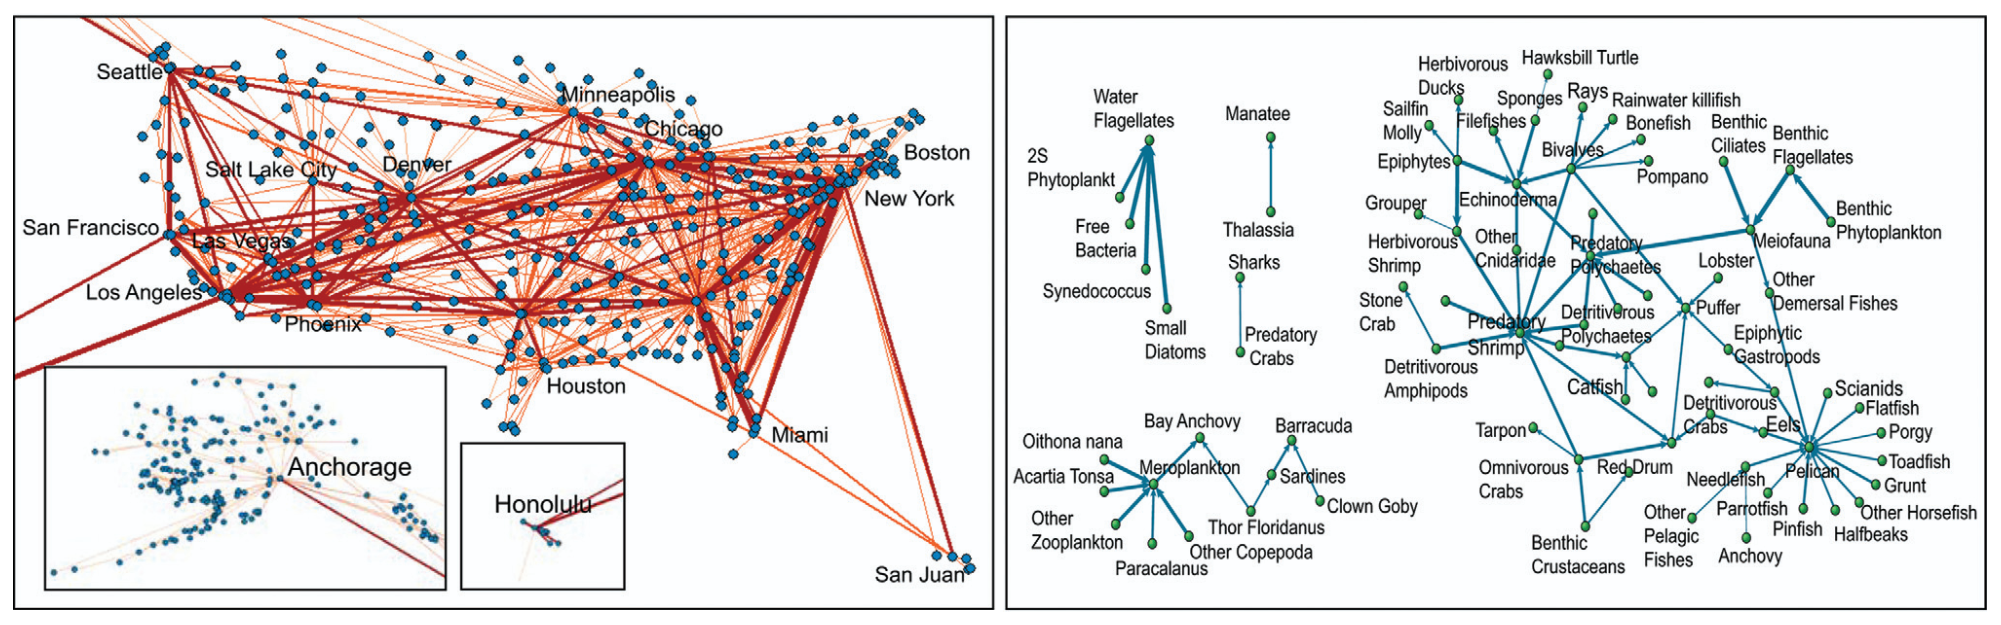
\includegraphics[width=0.8\textwidth]{img/disparity_backbone.png}
    \caption{Multiscale backbone extraction using the disparity filter. The left panel shows the backbone of the U.S. airport transportation system, while the right panel illustrates the backbone of the Florida Bay food web. In both cases, local filtering preserves the structural integrity of the network across different scales, highlighting critical connections that would be lost with global thresholding.}
\end{figure}

\section{Spectral Analysis of Networks}

Through the analysis of the eigenvalues and eigenvectors of matrices associated with a network, such as the adjacency matrix or the Laplacian matrix, we can gain insights into the structural properties of the network. Spectral analysis can reveal important information about the connectivity, community structure, and dynamics of the network. For example, the largest eigenvalue of the adjacency matrix can indicate the presence of hubs in the network, while the second smallest eigenvalue of the Laplacian matrix can provide information about the connectivity and robustness of the network. Spectral methods are widely used in various applications, including clustering, dimensionality reduction, and network visualization.

\subsection{The Eigenvalue Spectrum}
We can read the problem as an \textbf{eigenvalue problem}:
\[
    A \cdot \mathbf{x} = \lambda \cdot \mathbf{x},
\]
where \(A\) is the adjacency matrix of the network, \(\mathbf{x}\) is an eigenvector, and \(\lambda\) is the corresponding eigenvalue. The eigenvalues and eigenvectors can provide insights into the structure and properties of the network, such as identifying communities, detecting central nodes, and understanding the dynamics of processes on the network. Spectral analysis can also be used to identify important features of the network, such as its connectivity, robustness, and resilience to perturbations.

\begin{example}[Principal Component Analysis (PCA)]
    Principal Component Analysis (PCA) is a dimensionality reduction technique that can be applied to network data to identify the most important features or components that capture the variance in the data. By analyzing the eigenvalues and eigenvectors of the covariance matrix of the network data, PCA can help to identify patterns and relationships between nodes, as well as reduce the complexity of the data while preserving its essential structure. PCA can be particularly useful for visualizing high-dimensional network data and for identifying clusters or communities within the network.
\end{example}

We can also imply the \textbf{characteristic polynomial} of the adjacency matrix \(A\), defined as
\[
    \Phi(\lambda) = \det(A - \lambda \mathbb{I}),
\]
where \(I\) is the identity matrix. The roots of this polynomial are the eigenvalues of \(A\), and analyzing them can provide further insights into the structural properties of the network.

\subsection{Powers of the Adjacency Matrix}

Let us start by defining the powers of the adjacency matrix \(A\). The \(n\)-th power of the adjacency matrix, denoted as \(A^n\), can be computed using matrix multiplication. The entry \((A^n)_{ij}\) represents the number of paths of length \(n\) from node \(i\) to node \(j\) in the network:
\[
    B = A^2, \quad B_{ij} = \sum_{k} A_{ik} A_{kj}, \quad B_{ii} = \sum_{k} A_{ik} A_{ki}.
\]
This is because each multiplication of the adjacency matrix counts the number of ways to traverse from one node to another through intermediate nodes. This multiplication tells us how many paths of length \(n\) exist between nodes \(i\) and \(j\). For example, if \(A^2_{ij} > 0\), it means there is at least one path of length 2 (since we are looking at the second power) connecting nodes \(i\) and \(j\).

\(B_{ii}\) can infere on directed and undirected paths in the network, as it counts the number of paths that start and end at the same node \(i\). In an \textbf{undirected network}, this would count the number of loops or cycles that involve node \(i\), while in a \textbf{directed network}, it would count the number of directed paths that return to node \(i\). This information can be useful for understanding the local structure and connectivity of the network around node \(i\).

\begin{itemize}
    \item The first non-null term \(ij\) of the \(k\)-th power of \(A\) indicates the length of the shortest path from \(i\) to \(j\) (without specifying the route(s)).
    \item The k-th power matrix counts the number of walks from one node to another.
    \item If an element \(A^k_{ij} = 0\) for each \(k\), there are no paths between the two nodes (up to \(k_{\text{max}} = \#\text{nodes}\)).
    \item If the graph is directed, certain paths/walks may not exist.
    \item If no paths exist between two nodes in a symmetric graph, then the network is disconnected.
\end{itemize}

\subsection{Spectra of Specific Graphs}

\subsubsection{Cycles}

A \textit{directed cycle} ($C_{ND}$) is a path that starts and ends at the same node, strictly following the direction of the edges. If we multiply the adjacency matrix by itself $N$ times (where $N$ is the number of nodes), we return to the starting point, meaning:
\[
    (C_{ND})^N = \mathbb{I} \implies \lambda_i^N = 1 \implies \lambda_i = e^{i\frac{2\pi k}{N}} \quad \text{for } k = 0, 1, \ldots, N-1
\]
This shows that the eigenvalues of a directed cycle graph are exactly the $N$-th roots of unity, lying perfectly on the unit circle in the complex plane. For example, for $N=4$, the directed cycle matrix is:
\[
    C_{4D} = \begin{pmatrix}
        0 & 1 & 0 & 0 \\
        0 & 0 & 1 & 0 \\
        0 & 0 & 0 & 1 \\
        1 & 0 & 0 & 0
    \end{pmatrix}
\]

For an \textbf{undirected cycle network}, the adjacency matrix is simply the sum of the directed cycle and its transpose:
\[
    C_N = C_{ND} + C_{ND}^T
\]
A useful property of cycle matrices is that reversing the direction of the edges (taking the transpose) is mathematically equivalent to taking $N-1$ forward steps, meaning $C_{ND}^T = (C_{ND})^{N-1}$.

Because of this relationship, the eigenvalues of the undirected cycle are the sum of the eigenvalues of the directed cycle and their complex conjugates. This results in purely real periodic functions:
\[
    \lambda(C_N) = e^{i\frac{2\pi k}{N}} + e^{i\frac{2\pi k (N-1)}{N}} = 2\operatorname{Re}\left(e^{i\frac{2\pi k}{N}}\right) = 2\cos\left(\frac{2\pi k}{N}\right)
\]
For example, the adjacency matrix for an undirected cycle with $N=4$ nodes is perfectly symmetric and explicitly written as:
\[
    C_4 = \begin{pmatrix}
        0 & 1 & 0 & 1 \\
        1 & 0 & 1 & 0 \\
        0 & 1 & 0 & 1 \\
        1 & 0 & 1 & 0
    \end{pmatrix}
\]

\subsubsection{Completely Connected Graphs}

These graphs have a simple, dense structure where every node is directly connected to every other node.

If we consider an \textbf{all-ones matrix} (where even self-loops are included), the matrix has rank 1. It possesses a unique eigenvalue equal to $N$ (the number of nodes), corresponding to an eigenvector with all equal components. All other $N-1$ eigenvalues are exactly $0$.

However, a true completely connected graph ($K_N$) has no self-loops. Therefore, we must subtract the identity matrix to get zeros on the diagonal (meaning $\text{tr}(A) = 0$). The adjacency matrix looks like:
\[
    A = \begin{pmatrix}
        0      & 1      & 1      & \cdots & 1      \\
        1      & 0      & 1      & \cdots & 1      \\
        1      & 1      & 0      & \cdots & 1      \\
        \vdots & \vdots & \vdots & \ddots & \vdots \\
        1      & 1      & 1      & \cdots & 0
    \end{pmatrix}
\]
Subtracting the identity shifts the spectrum:
\begin{itemize}
    \item The first dominant eigenvalue becomes $N-1$ (reflecting that each node is connected to $N-1$ neighbors).
    \item The other $N-1$ eigenvalues become $-1$.
\end{itemize}
This highly symmetric spectrum with one massive eigenvalue and many identical negative eigenvalues characterizes perfectly dense cliques.

\subsubsection{Bipartite Graphs}

\begin{figure}[H]
    \begin{minipage}{0.45\textwidth}
        A bipartite graph consists of two distinct sets of nodes, where connections only exist \textit{between} the two sets, never within the same set.

        Topologically, this means the adjacency matrix can always be sorted and reduced to a \textbf{block off-diagonal form}:
        \[
            A = \begin{pmatrix}
                0        & B^1_{MN} \\
                B^2_{NM} & 0
            \end{pmatrix}
        \]
    \end{minipage}
    \hfill
    \begin{minipage}{0.5\textwidth}
        \centering
        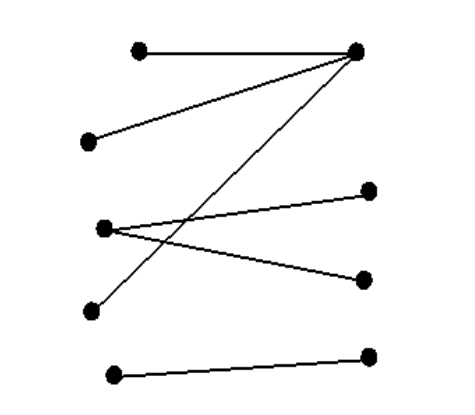
\includegraphics[width=0.8\textwidth]{img/bipartite_graph_spectral.png}
        \caption{Representation of a bipartite graph.}
    \end{minipage}
\end{figure}

Because you must always cross from set 1 to set 2 and back, \textbf{no odd-length cycles can exist}. Mathematically, the trace of any odd power of the adjacency matrix counts the number of odd cycles, so it must be zero:
\[
    \text{tr}(A^{2k+1}) = \sum_i \lambda_i^{2k+1} = 0 \quad \text{for } k = 0, 1, 2, \dots
\]
For this sum to always be zero, the \textbf{eigenvalue distribution must be perfectly symmetric} around zero (for every positive eigenvalue $\lambda$, there is a corresponding negative eigenvalue $-\lambda$).


\subsubsection{Directed Acyclic Graph (DAG)}

A Directed Acyclic Graph represents a strictly hierarchical structure where flow has a clear direction, and no closed loops exist.

Because there are no cycles, the nodes can be topologically sorted such that all links point strictly "forward". Consequently, its adjacency matrix can always be reduced to an \textbf{strictly upper triangular matrix} $U$:
\[
    A = \begin{pmatrix}
        0 & U \\
        0 & 0
    \end{pmatrix}
\]
A fundamental property of such a matrix is that it is \textbf{nilpotent}. Because the maximum possible walk length in a DAG without repeating a node is $N-1$ (the DAG diameter), taking the $N$-th power of the matrix evaluates to zero:
\[
    DAG^k = 0 \quad \forall k \geq N
\]
Physically, this means any process or random walk on a DAG will inevitably reach a "dead end" within $N$ steps.
\[
    N = \begin{bmatrix}
        0 & 2 & 1 & 6 \\
        0 & 0 & 1 & 2 \\
        0 & 0 & 0 & 3 \\
        0 & 0 & 0 & 0
    \end{bmatrix}; \quad
    N^2 = \begin{bmatrix}
        0 & 0 & 2 & 7 \\
        0 & 0 & 0 & 3 \\
        0 & 0 & 0 & 0 \\
        0 & 0 & 0 & 0
    \end{bmatrix}; \quad
    N^3 = \begin{bmatrix}
        0 & 0 & 0 & 6 \\
        0 & 0 & 0 & 0 \\
        0 & 0 & 0 & 0 \\
        0 & 0 & 0 & 0
    \end{bmatrix}; \quad
    N^4 = \begin{bmatrix}
        0 & 0 & 0 & 0 \\
        0 & 0 & 0 & 0 \\
        0 & 0 & 0 & 0 \\
        0 & 0 & 0 & 0
    \end{bmatrix}
\]

\subsubsection{Note on Cycles and Network Sparsity}
If a network has strictly no cycles, there is exactly a \textbf{single path} between any two nodes, which inherently corresponds to the shortest path. Such a network is formally a \textbf{tree}.

In the context of complex networks, this is an incredibly powerful approximation for \textbf{sparse networks}:
\begin{itemize}
    \item If a network has a very small number of links compared to the potential total ($o(N^2)$), cycles are mathematically rare, and long cycles are almost nonexistent.
    \item Because of this, when generating multiple paths between nodes in random network ensembles, cycles can often be considered negligible, effectively allowing us to treat sparse local neighborhoods as trees.
\end{itemize}
This "tree-like approximation" is the backbone of many analytical theorems in network science. Conversely, if we explicitly find many cycles in a highly sparse network, it serves as a strong \textbf{indicator of a specific, non-random structural design} (an evolutionary or engineered topology, rather than a random Erdős–Rényi graph).

\paragraph{Perturbations and Robustness}
What happens to the spectrum of these highly structured matrices if we slightly perturb the network? For example, if we add or remove a few edges or loops (altering cyclicity, destroying a strict bipartition, or breaking the all-ones symmetry), how does this affect the eigenvalues and eigenvectors?

This question is critical for understanding network robustness. Perturbations can be studied by randomly adding links/weights or by applying matrix perturbation theory. By observing how sensitive the spectral gap or the eigenvalue distribution is to these small topological changes, we can gain deep insights into the resilience of the network and its ability to maintain functionality (like diffusion or synchronization) under stress.

\subsection{Isomorphism and Spectral Analysis}

Two graphs are considered \textbf{isomorphic} if they are structurally identical and equal up to a simple node permutation (or node re-indexing). In matrix algebra, this corresponds to a transformation of similitude. If $A_1$ and $A_2$ are the adjacency matrices of two isomorphic graphs, they are related by a permutation matrix $P$ (where $P P^T = \mathbb{I}$):
\[
    A_1 = P A_2 P^T
\]
Taking the determinant of both sides proves that they share the exact same characteristic polynomial, and thus the exact same eigenvalues:
\[
    |A_1| = |P A_2 P^T| \implies |A_1| = |A_2|
\]
Graphs that share the exact same eigenvalue spectrum are called \textbf{cospectral}. The fundamental logical relations are:
\begin{itemize}
    \item \text{Isomorphic} $\implies$ \text{Cospectral}
    \item \text{Non-Cospectral} $\implies$ \text{Not Isomorphic}
\end{itemize}

However, the inverse is absolutely false: \textbf{co-spectrality DOES NOT imply isomorphism!} For graphs with $N > 4$ nodes (or "knots"), it is entirely possible to find two completely different, non-isomorphic network topologies that perfectly share the same spectrum.

This mathematical phenomenon was famously popularized by Mark Kac in his 1966 paper, \textit{"Can one hear the shape of a drum?"}. Just as two differently shaped drumheads can theoretically produce the exact same set of acoustic frequencies (eigenvalues), two differently wired networks can have the exact same spectrum.

\begin{figure}[H]
    \centering
    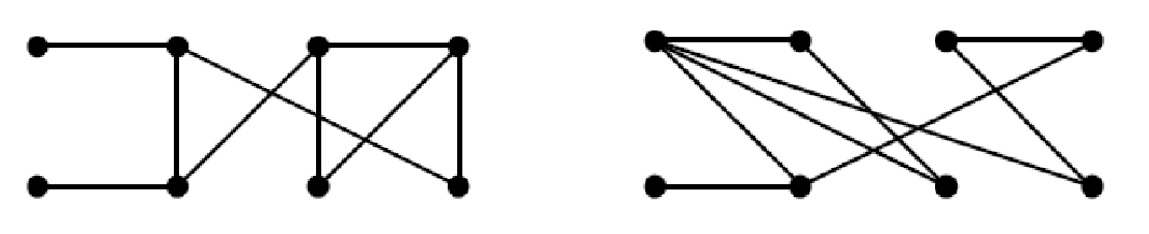
\includegraphics[width=0.8\textwidth]{img/cospectral_graphs.png}
    \caption{Two non-isomorphic graphs that are perfectly co-spectral. Despite their different topologies, they share the same eigenvalue spectrum, illustrating the concept of co-spectrality and the limitations of spectral analysis in uniquely identifying graph structures.}
\end{figure}

\subsubsection{Summary of Spectral Analysis}
To summarize the key points of network spectral analysis:
\begin{itemize}
    \item \textbf{Spectrum as a Summary:} The eigenvalue spectrum acts as a "summary" or defines the vibrational "modes" of a graph. It tells us about the global structure, but not all the microscopic information (it does not uniquely pinpoint specific arrangements or motifs due to the existence of cospectral graphs).
    \item \textbf{Representation Independence:} The spectrum is strictly invariant to how we label or draw the graph (node re-indexing).
    \item \textbf{Permutation Invariance:} Because node re-labeling is merely a similarity transform (involving a matrix and its inverse), the eigenvalue problem remains mathematically identical, dictated by the properties of the determinant of matrix products.
    \item \textbf{Analytical Limits:} There are few exact analytical results for general complex graphs. Most exact solutions are limited to particular cases (like trees or complete graphs), while general graphs rely heavily on numerical results.
\end{itemize}

\subsubsection{Co-spectrality: Adjacency vs. Laplacian Matrices}

When analyzing a network, we can choose different mathematical representations (e.g., the Adjacency matrix $A$ or the Laplacian matrix $L$). These matrices describe the exact same physical network but have completely different eigenvalue spectra.

A critical question arises: do they suffer from the same rate of co-spectrality? \textbf{NO!} \textit{(Reference: Wilson paper on Virtuale)}.

Empirical evidence on small networks (specifically trees) reveals a drastic difference in their identifying power:
\begin{itemize}
    \item \textbf{Adjacency Matrix ($A$):} The fraction of $A$-cospectral trees is surprisingly high. For small graphs (around 10-15 vertices), up to $\sim 30\%$ of non-isomorphic trees can share the exact same Adjacency spectrum. It is a relatively weak "fingerprint".
    \item \textbf{Laplacian Matrix ($L$):} The fraction of $L$-cospectral trees is drastically lower. For the same number of vertices, the peak fraction of non-isomorphic trees sharing a Laplacian spectrum is only about $\sim 2.5\%$.
\end{itemize}

This mathematically demonstrates that the Laplacian spectrum retains far more unique structural information than the Adjacency spectrum, making it a much more robust tool for distinguishing different network topologies.

\begin{figure}[H]
    \centering
    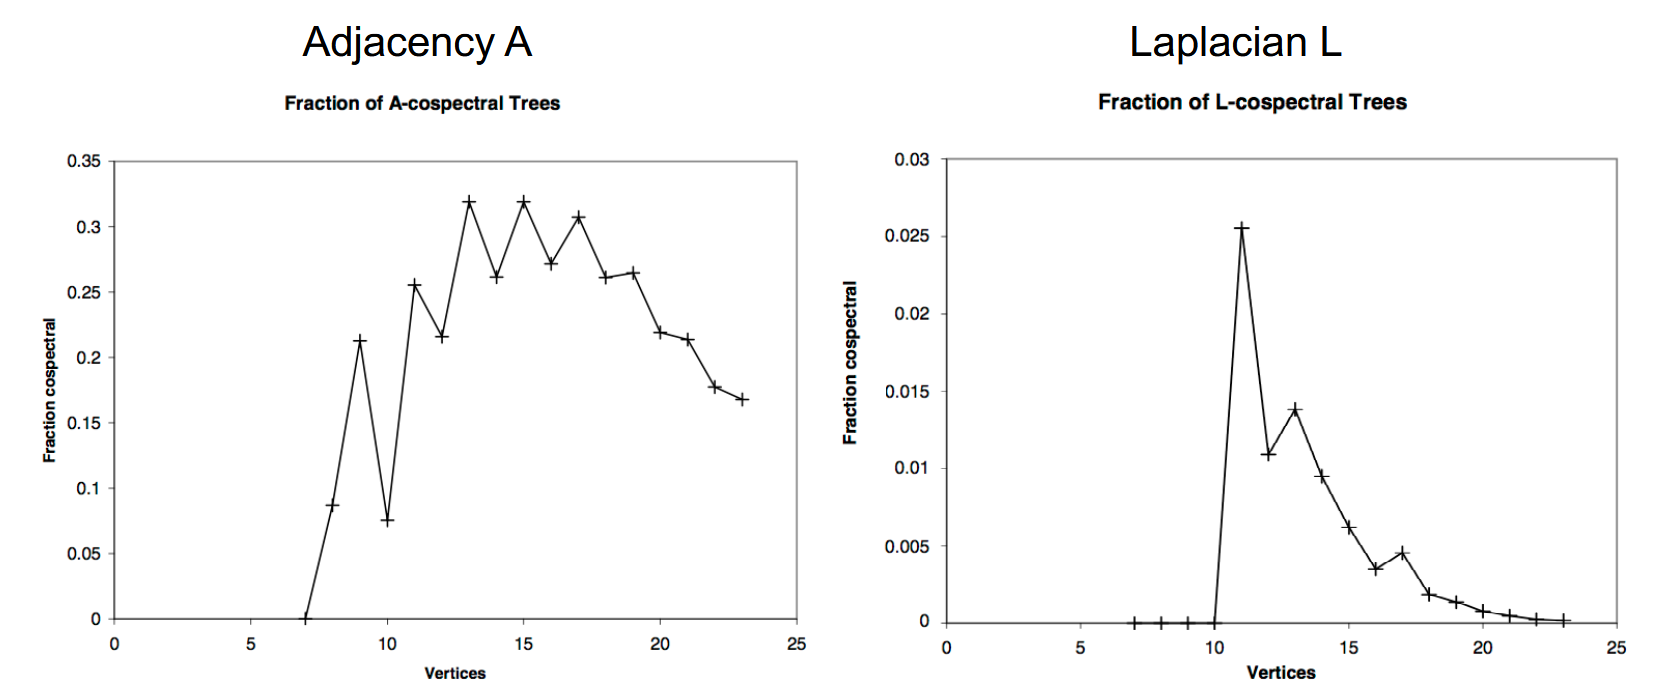
\includegraphics[width=0.8\textwidth]{img/cospectrality_comparison.png}
    \caption{Comparison of co-spectrality rates for Adjacency and Laplacian matrices in trees. The left panel shows the fraction of $A$-cospectral trees, peaking at around 30\%, while the right panel shows the fraction of $L$-cospectral trees, peaking at only about 2.5\%. This stark contrast highlights the superior discriminative power of the Laplacian spectrum in capturing unique structural features of networks.}
\end{figure}

\subsection{Graph Distances}

When comparing two networks, we need a robust mathematical measure to define how "similar" they are. This can be approached in two primary ways: by comparing their algebraic representations (\textbf{Spectral Distance}) or by comparing their physical topologies (\textbf{Graph Edit Distance}).

\subsubsection{Graph Spectral Distance}
The spectral distance evaluates the similarity of two graphs by comparing their eigenvalue spectra.

To calculate this, the eigenvalues of both graphs must first be sorted. If the two networks have a different number of nodes ($N_1 \neq N_2$), we must mathematically align their dimensions by adding zeros to the smaller spectrum. Physically, this \textbf{zero-padding} corresponds to adding isolated nodes to the network, which do not contribute to the active spectrum calculation.
\[
    \begin{aligned}
        \lambda_1 \leq \lambda_2 \leq \ldots \leq \lambda_N \\
        \mu_1 \leq \mu_2 \leq \ldots \leq \mu_N
    \end{aligned}
\]
The spectral distance $d(G_1, G_2)$ is defined as the Euclidean distance between these sorted, zero-padded eigenvalue vectors:
\[
    d(G_1, G_2) = \sqrt{\sum_{i=1}^N (\lambda_i - \mu_i)^2}
\]
A fundamental property of this measure is that the spectral distance is \textbf{strictly invariant to node index permutation}. This makes it extremely useful: even if two identical graphs are labelled completely differently, their spectral distance will correctly be zero.

\subsubsection{Graph Edit Distance (GED)}
While spectral distance operates in the algebraic domain, the \textbf{Graph Edit Distance} operates directly on the topology. It is defined as the minimum number of elementary "steps" (specifically, edge additions or edge removals) required to transform one graph into another.

\textit{Crucial Note:} In this framework, adding or removing an \textbf{isolated node} has absolutely zero weight (it also has zero weight on the active spectrum). Only the modification of \textbf{links} contributes to the distance.

\begin{example}[Calculating Graph Edit Distance]
    Consider three simple graphs made of a few nodes connected in different topologies:
    \begin{itemize}
        \item To switch from Graph 1 (a closed square) to Graph 3 (an open line), we only need to remove exactly one link. Thus, the distance is $d = 1$.
        \item To switch from Graph 2 (a star-like structure) to Graph 3, we must remove one specific link and add a different one. Thus, $d = 2$.
        \item To switch from Graph 1 to Graph 2, we must remove two links and add one. Thus, $d = 3$.
    \end{itemize}
\end{example}

\begin{figure}[H]
    \centering
    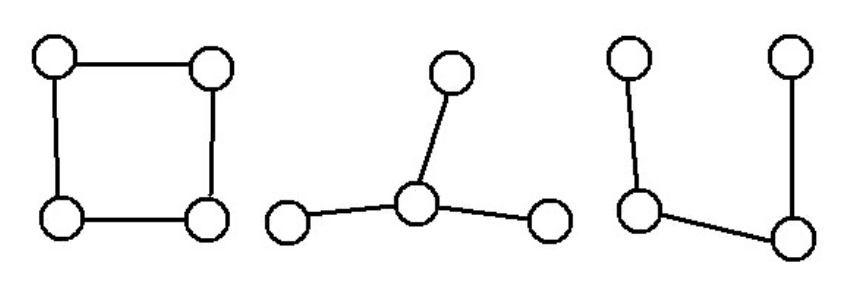
\includegraphics[width=0.8\textwidth]{img/graph_edit_distance.png}
    \caption{Illustration of Graph Edit Distance (GED) between three simple graphs. The left panel shows the original graphs, while the right panel highlights the specific edge modifications required to transform one graph into another, along with the corresponding edit distances (d=1, d=2, d=3). This visual representation helps to clarify how GED quantifies topological differences between networks.}
\end{figure}

\paragraph{Parallel with Bioinformatics}
Graph edit distance is a direct generalization of the \textbf{edit distance between strings of symbols}, heavily used in bioinformatics (protein/DNA sequences) and text analysis (words/periods).

In symbol sequences, elementary operations include \textit{symbol substitution}, \textit{insertion}, or \textit{removal}. The sequence of operations connecting one string to another can be represented in a graph table, where a path represents the editing steps. To identify the best matching between two sequences, different scoring systems are defined, such as:
\begin{itemize}
    \item Finding the \textbf{Longest Common Subsequence} (which translates to the maximum common subgraph in network theory).
    \item Calculating \textbf{Global alignment scores} based on varying penalty values associated with mismatches, insertions, or deletions.
\end{itemize}

\begin{example}[DNA Sequences vs. Networks]
    For proteins and DNA sequences, there is a \textbf{natural node ordering} (the 1D sequence of the molecule). Because of this strict ordering, calculating string edit distance is computationally straightforward.

    For complex networks, however, there is \textbf{no natural node ordering}. Finding the correct starting point for node-to-node mapping is highly nontrivial (this is the Graph Matching Problem). To solve this, researchers explore open approaches such as:
    \begin{itemize}
        \item \textbf{Spectral approaches:} Using matrix eigenvector components to identify node similarities.
        \item Evaluating similarities between modern \textbf{node embeddings}.
    \end{itemize}
\end{example}

\subsubsection{Correlation: Spectra vs. Topology}
A fundamental finding in modern network science is that there is a \textbf{strong linear correlation} between the algebraic Spectral Distance and the topological Graph Edit Distance.

If we take a graph and progressively delete edges, plotting the number of deleted edges against the resulting Euclidean spectral distance reveals a clear, monotonically increasing line. This holds true whether we use the Adjacency matrix or the standard Laplacian matrix.
Therefore, proximity in the eigenvalue spectra deeply reflects graphs with highly similar physical structures, validating spectral analysis as a powerful tool for comparing networks (even if specific, non-isomorphic exceptions exist).

\begin{figure}[H]
    \centering
    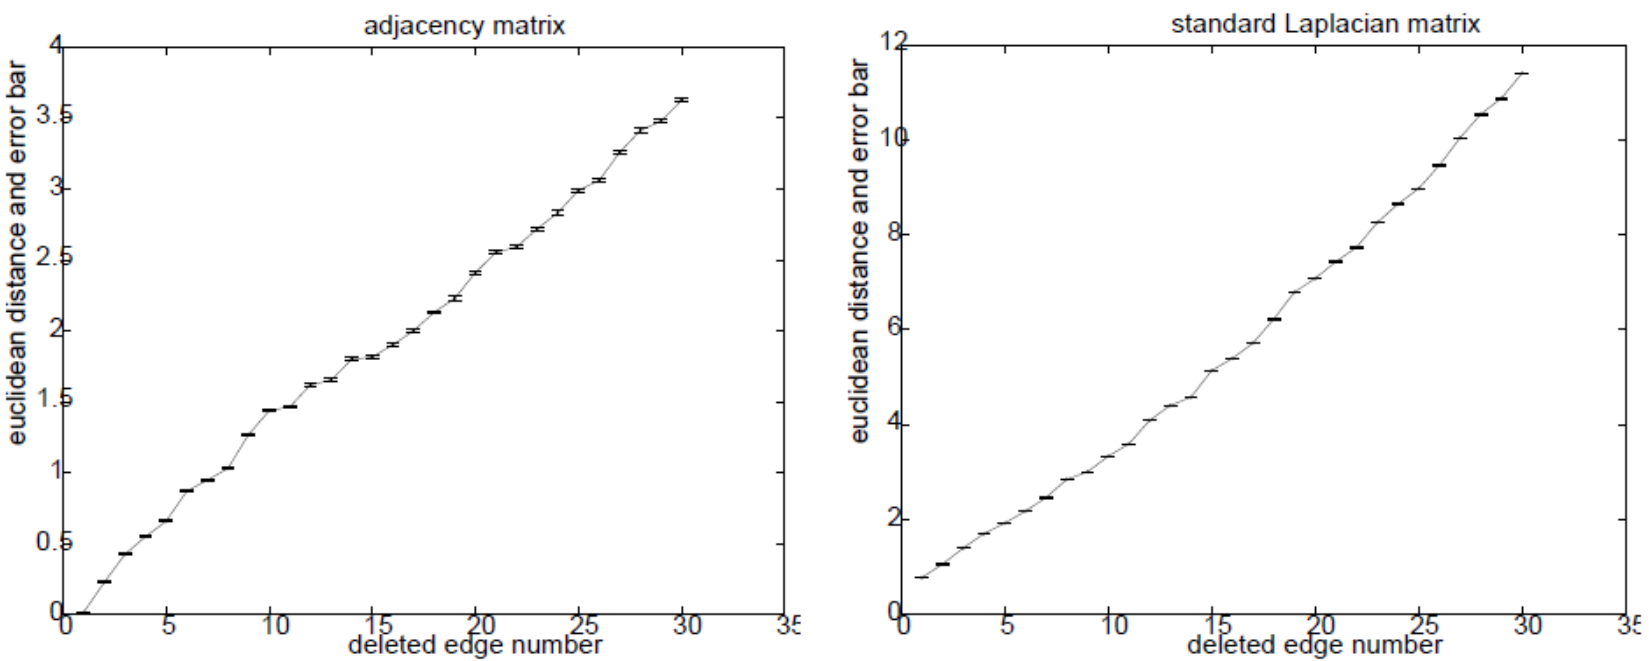
\includegraphics[width=0.8\textwidth]{img/spectral_vs_topological_distance.png}
    \caption{Scatter plots showing the relationship between the number of deleted edges (Graph Edit Distance) and the Euclidean spectral distance for both the Adjacency matrix and the standard Laplacian matrix. The plots reveal a strong linear correlation, indicating that as more edges are deleted (increasing topological distance), the spectral distance also increases, demonstrating the effectiveness of spectral analysis in capturing structural differences between graphs.}
\end{figure}